\documentclass[pdf]{beamer}
%\mode<presentation>{}

\usepackage{amssymb,amsmath,amsthm,enumerate,mathtools}
\usepackage[utf8]{inputenc}
\usepackage{array}
\newcolumntype{C}[1]{>{\centering\arraybackslash}m{#1}}

\usepackage[parfill]{parskip}
\usepackage{graphicx}
\usepackage{caption}
\captionsetup[figure]{labelformat=empty}
\usepackage{subcaption}
\usepackage{bm}
\usepackage{amsfonts,amscd}
%\usepackage{gensymb}
\usepackage[]{units}
\usepackage{listings}
\usepackage{multicol}
\usepackage{tcolorbox}
\usepackage{physics}
\usepackage{multirow}
\usepackage{pgfplots,tikz}
\pgfplotsset{compat=1.7}
\usepackage{hyperref}
\hypersetup{
    colorlinks=true,
    linkcolor=franklinblue,
    filecolor=magenta,      
    urlcolor=cyan,
    bookmarks=true,
    citecolor= black
    % pdftitle={Overleaf Example},
    % pdfpagemode=FullScreen,
    }
\usepackage{colortbl}
\usepackage{booktabs}
\usepackage{gensymb}
\usepackage{color}
\usepackage{natbib}

\usepackage{tikz}
\usepackage{fixltx2e}
\usepackage[english]{babel}
\usepackage[absolute,overlay]{textpos}
%\usepackage{gnuplottex} % For t-distribution using gnuplot.
%The following function is use in students t distribution. 
% \def\basefunc{    gamma((\n+1)/2.)/(sqrt(\n*pi)*gamma(\n/2.))*((1+(x*x)/\n)^(-(\n+1)/2.))}    
% \def\n{7}
%\usepackage{tkz-fct} % For t-distribution plotting.
% \usepackage{pst-func} % For t-distribution plotting.
\usepackage{longtable}
\usepackage{changepage} 

\usetikzlibrary{shapes,decorations,arrows,calc,arrows.meta,fit,positioning}
\tikzset{
    -Latex,auto,node distance =1 cm and 1 cm,semithick,
    state/.style ={ellipse, draw, minimum width = 0.7 cm},
    point/.style = {circle, draw, inner sep=0.04cm,fill,node contents={}},
    bidirected/.style={Latex-Latex,dashed},
    el/.style = {inner sep=2pt, align=left, sloped}
}

%Normal Distribution
\pgfmathdeclarefunction{gauss_}{2}{\pgfmathparse{1/(#2*sqrt(2*pi))*exp(-((x-#1)^2)/(2*#2^2))}%
}
%Gamma Distribution
\pgfmathdeclarefunction{gammaPDF}{2}{
\pgfmathparse{1/(#2^#1*gamma(#1))*x^(#1-1)*exp(-x/#2)}
}

%%%%% For https://tikz.net/gaussians/ %%%%%

\usepackage{amsmath} % for \dfrac
\usepackage{tikz}
\tikzset{>=latex} % for LaTeX arrow head
\usepackage{pgfplots} % for the axis environment
\usepackage{xcolor}
\usepackage[outline]{contour} % halo around text
\contourlength{1.2pt}
\usetikzlibrary{positioning,calc}
\usetikzlibrary{backgrounds}% required for 'inner frame sep'
%\usepackage{adjustbox} % add whitespace (trim)

% define gaussian pdf and cdf
\pgfmathdeclarefunction{gauss}{3}{%
  \pgfmathparse{1/(#3*sqrt(2*pi))*exp(-((#1-#2)^2)/(2*#3^2))}%
}
\pgfmathdeclarefunction{cdf}{3}{%
  \pgfmathparse{1/(1+exp(-0.07056*((#1-#2)/#3)^3 - 1.5976*(#1-#2)/#3))}%
}
\pgfmathdeclarefunction{fq}{3}{%
  \pgfmathparse{1/(sqrt(2*pi*#1))*exp(-(sqrt(#1)-#2/#3)^2/2)}%
}
\pgfmathdeclarefunction{fq0}{1}{%
  \pgfmathparse{1/(sqrt(2*pi*#1))*exp(-#1/2))}%
}

\colorlet{mydarkblue}{blue!30!black}

% to fill an area under function
\usepgfplotslibrary{fillbetween}
\usetikzlibrary{patterns}
\pgfplotsset{compat=1.12} % TikZ coordinates <-> axes coordinates
% https://tex.stackexchange.com/questions/240642/add-vertical-line-of-equation-x-2-and-shade-a-region-in-graph-by-pgfplots

% plot aspect ratio
%\def\axisdefaultwidth{8cm}
%\def\axisdefaultheight{6cm}

% number of sample points
\def\N{50}

%%%%% End for https://tikz.net/gaussians/ %%%%%

\setbeamertemplate{caption}[numbered]

%new commands
\newcommand{\der}[2]{\frac{d#1}{d#2}}
\newcommand{\nder}[3]{\frac{d^#1 #2}{d #3 ^ #1}}
\newcommand{\pder}[2]{\frac{\partial #1}{\partial #2}}
\newcommand{\npder}[3]{\frac{\partial ^#1 #2}{\partial #3^#1}}
\newcommand{\sentencelist}{def}
\newcommand{\overbar}[1]{\mkern 1.5mu\overline{\mkern-1.5mu#1\mkern-1.5mu}\mkern 1.5mu}
\newcommand{\lined}{\overbar}
\newcommand{\perm}[2]{{}^{#1}\!P_{#2}}
\newcommand{\comb}[2]{{}^{#1}C_{#2}}
\newcommand{\intall}{\int_{-\infty}^{\infty}}
\newcommand{\Var}[1]{\text{Var}\left(#1\right)}
\newcommand{\E}[1]{\text{E}\left(#1\right)}
\newcommand{\define}{\equiv}
\newcommand{\diff}[1]{\mathrm{d}#1}
\newcommand{\empy}[1]{{\color{cadetblue}\texttt{#1}}}
\newcommand{\empr}[1]{{\color{franklinblue}\textbf{#1}}}
%https://tex.stackexchange.com/questions/192358/quickly-changing-all-the-file-paths-in-a-tex-file
%\newcommand{\pathtopdf}{C:/Users/bkwei/OneDrive - Franklin University/Desktop/Math_215/Data/IMDB/Processed} - Not Tested!
\newcolumntype{L}[1]{>{\raggedright\let\newline\\\arraybackslash\hspace{0pt}}m{#1}}
\newcolumntype{C}[1]{>{\centering\let\newline\\\arraybackslash\hspace{0pt}}m{#1}}
\newcolumntype{R}[1]{>{\raggedleft\let\newline\\\arraybackslash\hspace{0pt}}m{#1}}

\theoremstyle{remark}
\newtheorem*{remark}{Remark}
\theoremstyle{definition}

\newcommand{\examplebox}[2]{
\begin{tcolorbox}[colframe=darkcardinal,colback=boxgray,title=#1]
\end{tcolorbox}}

\newcommand{\eld}[1]{\frac{d}{dt}(\frac{\partial L}{\partial \dot #1}) - \frac{\partial L}{\partial #1}=0}
\newcommand{\euler}[1]{\frac{\partial L}{\partial #1}-\frac{d}{dt}(\frac{\partial L}{\partial \dot #1})}
\newcommand{\eulerg}[1]{\frac{\partial g}{\partial #1}-\frac{d}{dt}(\frac{\partial g}{\partial \dot #1})}
\newcommand{\divg}[1]{\nabla\cdot #1}
\newcommand{\prob}[1]{P(#1\vert I)}

\AtBeginSection[]{
  \begin{frame}
  \vfill
  \centering
  \begin{beamercolorbox}[sep=8pt,center,%shadow=true,
  rounded=true]{section}
    \LARGE
    \usebeamerfont{section}
    %\usebeamercolor[fg]{section}\inserttitle %\insertsectionhead\par%
    \setbeamercolor{section}{fg=white,bg=white}\insertsectionhead\par%
  \end{beamercolorbox}
  \vfill
  \end{frame}
}

\usetheme{Franklin} 
\def \i  {\item}
\def \ai {\item[] \quad \arrowbullet}
\newcommand \si[1]{\item[] \quad \bulletcolor{#1}}
\def \wi {\item[] \quad $\ \phantom{\Rightarrow}\ $}
\def \bi {\begin{itemize}\item}
\def \ei {\end{itemize}}
\def \be {\begin{equation*}}
\def \ee {\end{equation*}}
\def \bie {$\displaystyle{}
\def \eie {{\ }$}}
\def \bsie {\small$\displaystyle{}
\def \esie {{\ }$}\normalsize\selectfont}
\def \bse {\small\begin{equation*}}
\def \ese {\end{equation*}\normalsize}
\def \bfe {\footnotesize\begin{equation*}}
\def \efe {\end{equation*}\normalsize}
\renewcommand \le[1] {\\ \medskip \lefteqn{\hspace{1cm}#1} \medskip}
\def \bex {\begin{example}}
\def \eex {\end{example}}
\def \bfig {\begin{figure}}
\def \efig {\end{figure}}
\def \btheo {\begin{theorem}}
\def \etheo {\end{theorem}}
\def \bc {\begin{columns}}
\def \ec {\end{columns}}
\def \btab {\begin{tabbing}}
\def \etab {\end{tabbing}\svneg\svneg}
\newcommand \col[1]{\column{#1\linewidth}}
\def\vneg  {\vspace{-5mm}}
\def\lvneg {\vspace{-10mm}}
\def\svneg {\vspace{-2mm}}
\def\tvneg {\vspace{-1mm}}
\def\vpos  {\vspace{5mm}}
\def\lvpos {\vspace{10mm}}
\def\svpos {\vspace{2mm}}
\def\tvpos {\vspace{1mm}}
\def\hneg  {\hspace{-5mm}}
\def\lhneg {\hspace{-10mm}}
\def\shneg {\hspace{-2mm}}
\def\thneg {\hspace{-1mm}}
\def\hpos  {\hspace{5mm}}
\def\lhpos {\hspace{10mm}}
\def\shpos {\hspace{2mm}}

\logo{
\includegraphics[height=0.4in]{./style_files_franklin/FranklinUniversity_TM1.jpg}}

\title{BUSA 603}
\subtitle{Module 3 Supplement \\  Data Visualization \& Some Useful Charts}

\beamertemplatenavigationsymbolsempty

\begin{document}

\author[B. Weikel, Franklin University]{
	\begin{tabular}{c} 
	\Large
	Brian Weikel\\
    \footnotesize \href{mailto:brian.weikel@franklin.edu}{brian.weikel@franklin.edu}
    \vspace{1ex}
\end{tabular}
\vspace{-4ex}}

\institute{
	
\includegraphics[height=0.4in]{./style_files_franklin/FranklinUniversity_TM1.jpg}\\
	Business Analytics\\
	Franklin University}

\date{Spring 2024}%{\today}

\begin{noheadline}
\begin{frame}[t]\maketitle\end{frame}
\end{noheadline}

\begin{frame}[t]{Know Your Audience}
The first step in trying to interpret data is often to visualize it in some way. Data visualization can be as simple as creating a summary table, or it could require generating charts to help interpret, analyze, and learn from the data. \\
\vspace{0.5ex} 
\small
\begin{itemize}
\item Data visualization is very helpful for  identifying data errors and for reducing the size of your data set by highlighting important relationships and trends. \\
\item Data visualization is also important in conveying your analysis to others. Although business analytics is about making better decisions, in many cases, the ultimate decision maker is not the person who analyzes the data. 
\item When preparing for presentations that summarize data, always know your audience.  This will ensure that you are conveying the proper content that does not ``insult the intelligence'' of the audience. 
\end{itemize}
\end{frame}

\begin{frame}[t]{Determining If a Table or Chart is More Effective}
The first decision in displaying data is whether a table or a chart will be more effective. In general, charts can often convey information faster and easier to readers, but in some cases
a table is more appropriate. Tables should be used when:  \\
\vspace{1.5ex}
\begin{itemize}
\item The reader needs to refer to specific numerical values.
\item The reader needs to make precise comparisons between different values and not just
relative comparisons.
\item The values being displayed have different units or very different magnitudes.
\end{itemize}
\end{frame}

\begin{frame}[t]{Data-Ink Ratio}
\cite{tufte2001} recommends using the \empr{data-ink ratio} idea when creating effective designs.
\vspace{0.0ex}
\begin{enumerate}
\item The data-ink ratio measures the proportion of what Tufte terms ``data-ink'' to the total amount of ink used in a table or chart. 
\begin{itemize}
\item \empr{Data-ink} is the ink used in a table or chart that is necessary to convey the meaning of the data to the audience. 
\item \empr{Non-data-ink} is ink used in a table or chart that serves no useful purpose in conveying the data to the audience.
\end{itemize} 
\item This idea implies one should avoid using vertical lines in a table unless they are necessary for clarity.
\end{enumerate}
\end{frame}

\begin{frame}[t]{Horizontal and Vertical Line Recommendations}
\begin{enumerate}
  \setcounter{enumi}{2}
\item Horizontal lines are generally necessary only for separating column titles from data values or when indicating that a calculation has taken place.
\item In large tables, vertical lines or light shading can be useful to help the reader differentiate the columns and rows.
\item Since there may be audience members who are color-blind, use colors only when other data and text distinguishing options -- mark type, line size, line type, italic font, bold font \ldots -- have been exhausted.
\end{enumerate}
\end{frame}

\begin{frame}[t]{Graph Recommendations for Effective Presentations}
\cite{anderson2013}, \cite{lortie2017}, and \cite{naegle2021}, to name just a few, give advice on creating presentations with visualizations. \\
\vspace{1.5ex}
\begin{itemize}
\item  Build presentation slides around good visualizations. Remember, a picture is worth a thousand words. However, on the flip side, do not muddy the point of the slide by putting too many complex graphics on a single slide. 
\item Thus, use simple visuals.
\item Repeat \underline{critical messages} (at least) twice using different visuals.
\item Use the principle of parsimony in explanations of visualizations.
\end{itemize}
\end{frame}

\begin{frame}[t]{A Few Chart Types}
\begin{description}
\item [Scatter Chart] A chart that has two value axes: a horizontal ($x$) and a vertical ($y$) value axis. It combines $x$ and $y$ values into single data points and shows them in irregular intervals, or clusters. These charts are typically used for showing and comparing numeric values, like scientific, statistical, and engineering data.\footnote{\href{https://support.microsoft.com/en-us/office/available-chart-types-in-office-a6187218-807e-4103-9e0a-27cdb19afb90}{This Microsoft page} has information about chart types available in their software solutions.}
\item [Line Chart] A chart where category data is distributed evenly along the horizontal axis, and all value data is distributed evenly along the vertical axis. This chart can show continuous data over time on an evenly scaled axis, so they are ideal for showing trends in data at equal intervals, like months, quarters, or fiscal years.
\end{description}
\end{frame}

\begin{frame}[t]{A Scatter Chart Example}
%https://tex.stackexchange.com/questions/114908/change-position-of-figure-in-beamer
\begin{figure}[htbp]
  \centering
  \captionsetup{justification=centering}
  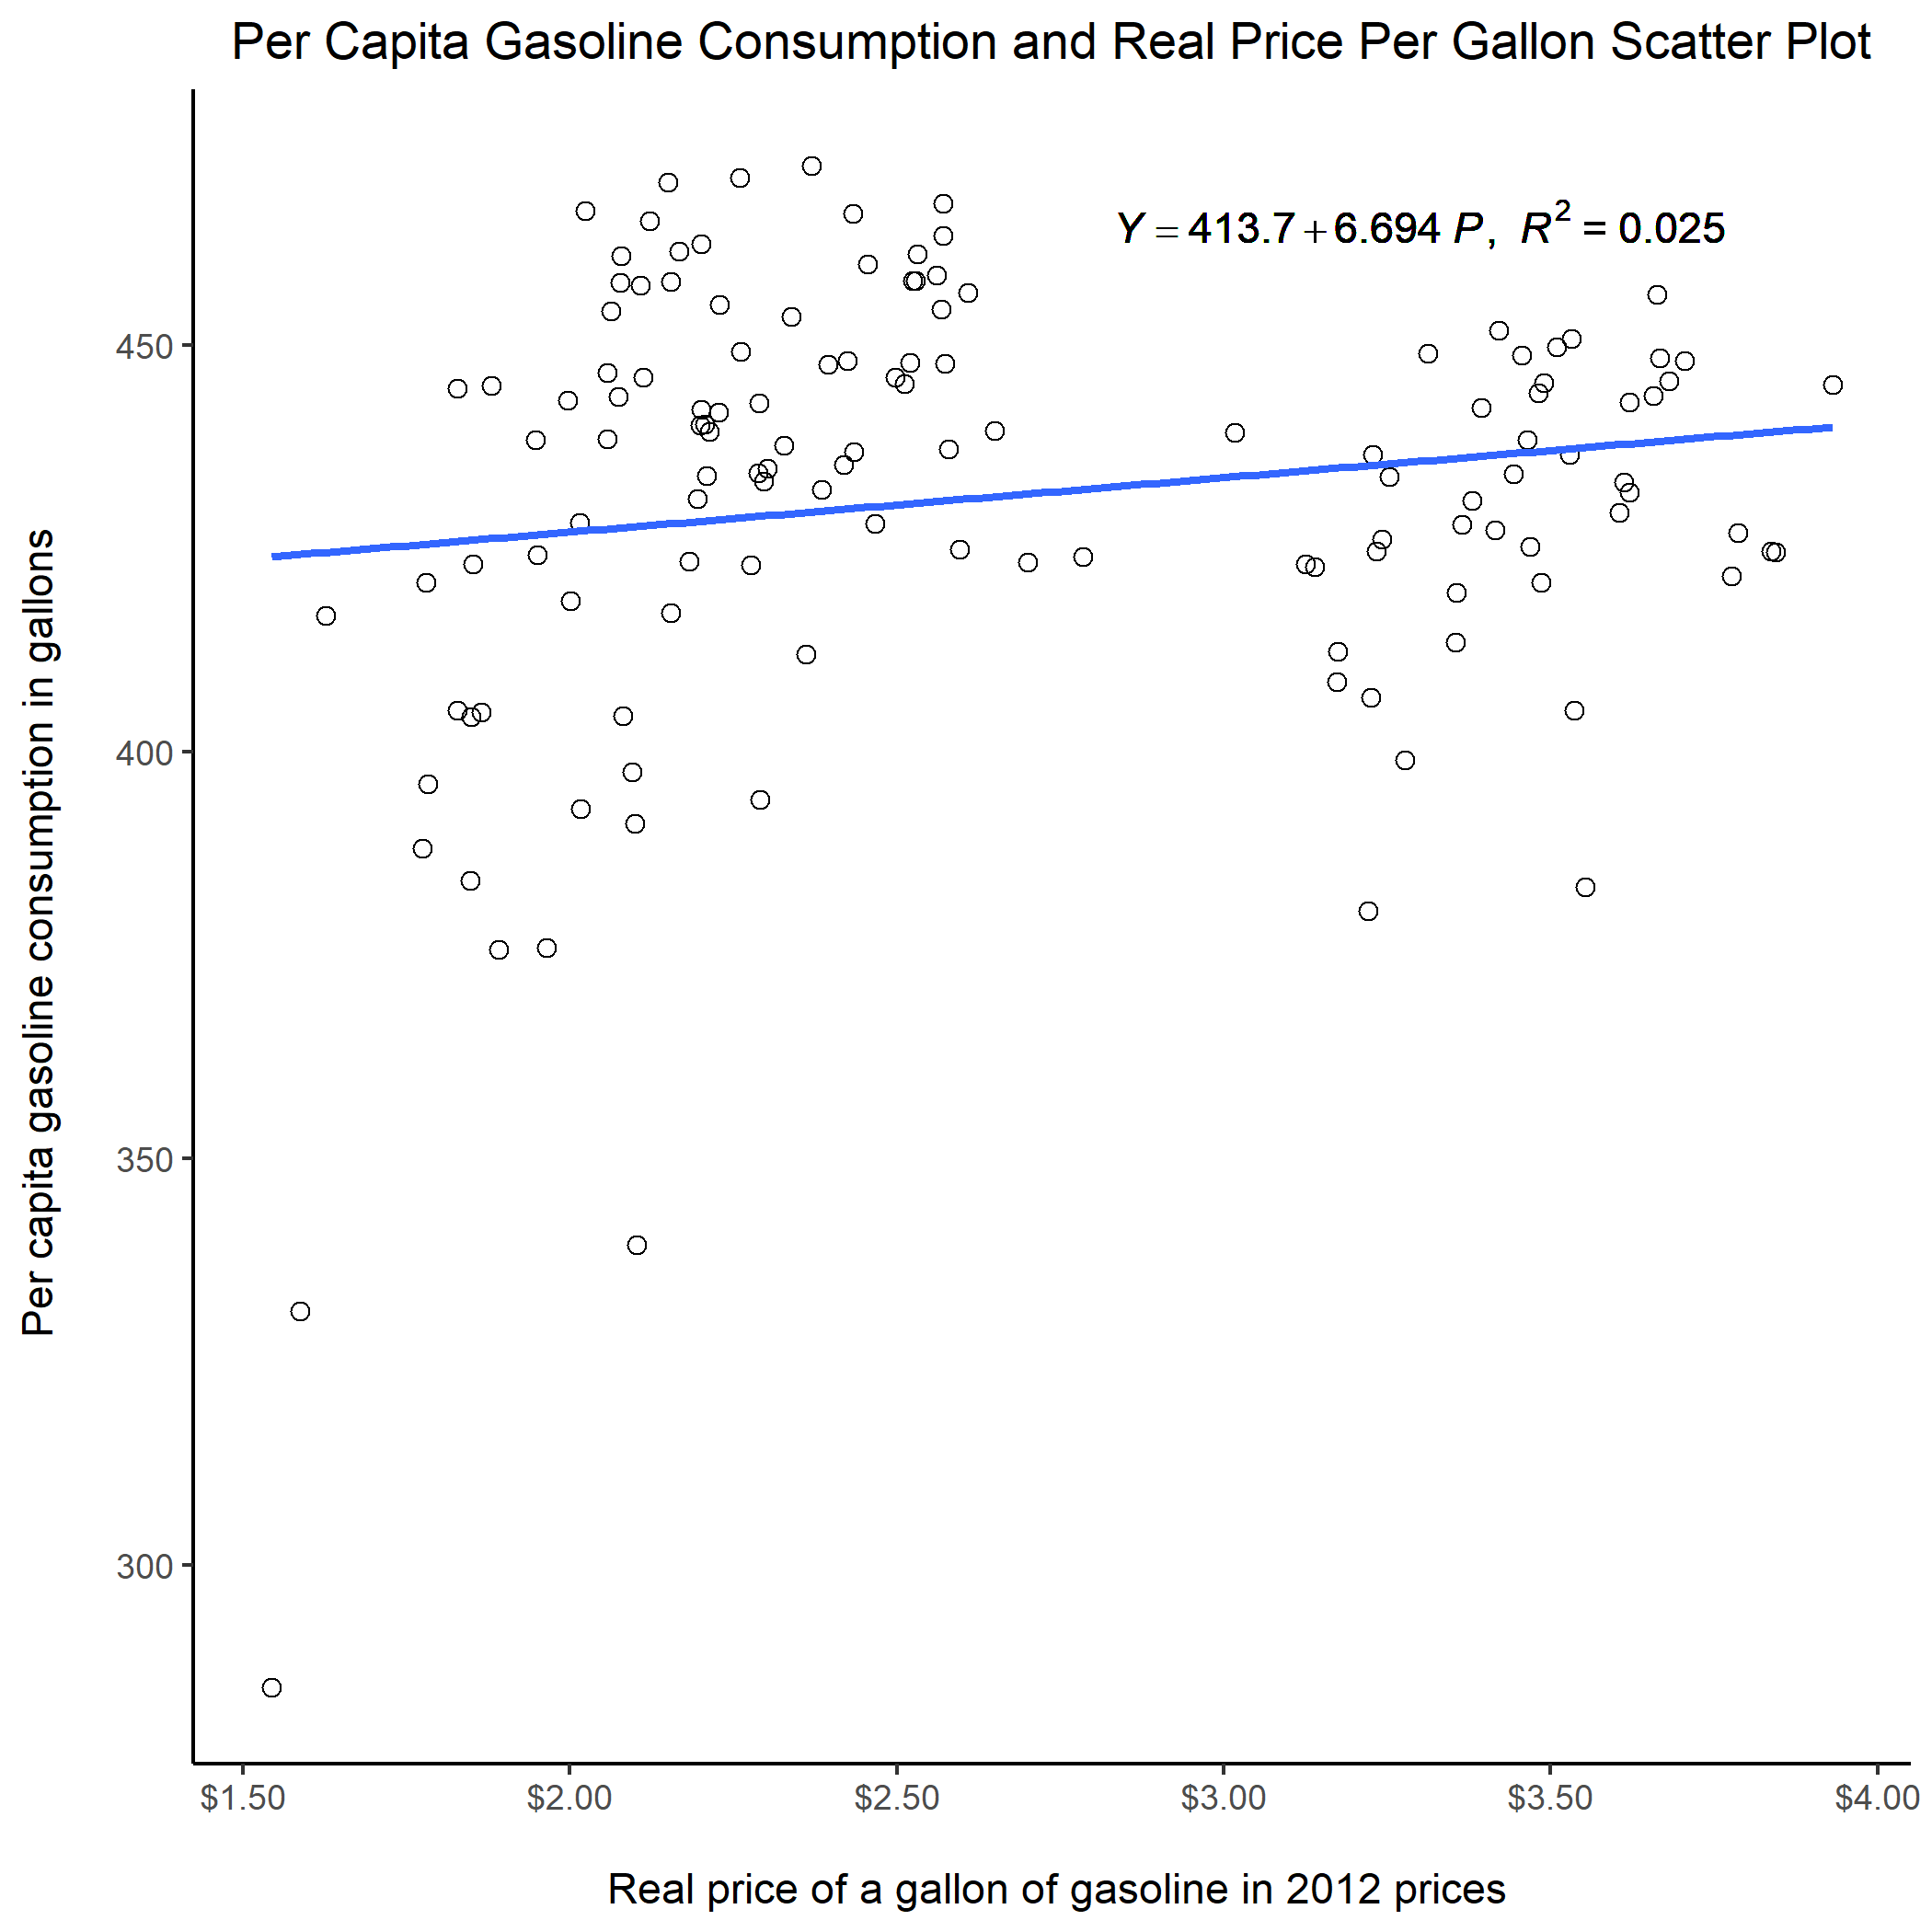
\includegraphics[clip, trim=0cm 0cm 0cm 0cm, width=0.6\textwidth]{Images/a1_q1c.png}
  \caption{Figure {\color{franklinblue} 1}: A Petroleum Distillate Demand and Real Price Scatter Chart}  
  \label{fig:scatterchart}
\end{figure}
\end{frame}

\begin{frame}[t]{A Line Chart Example}
%https://tex.stackexchange.com/questions/114908/change-position-of-figure-in-beamer
\begin{figure}[htbp]
  \centering
  \captionsetup{justification=centering}
  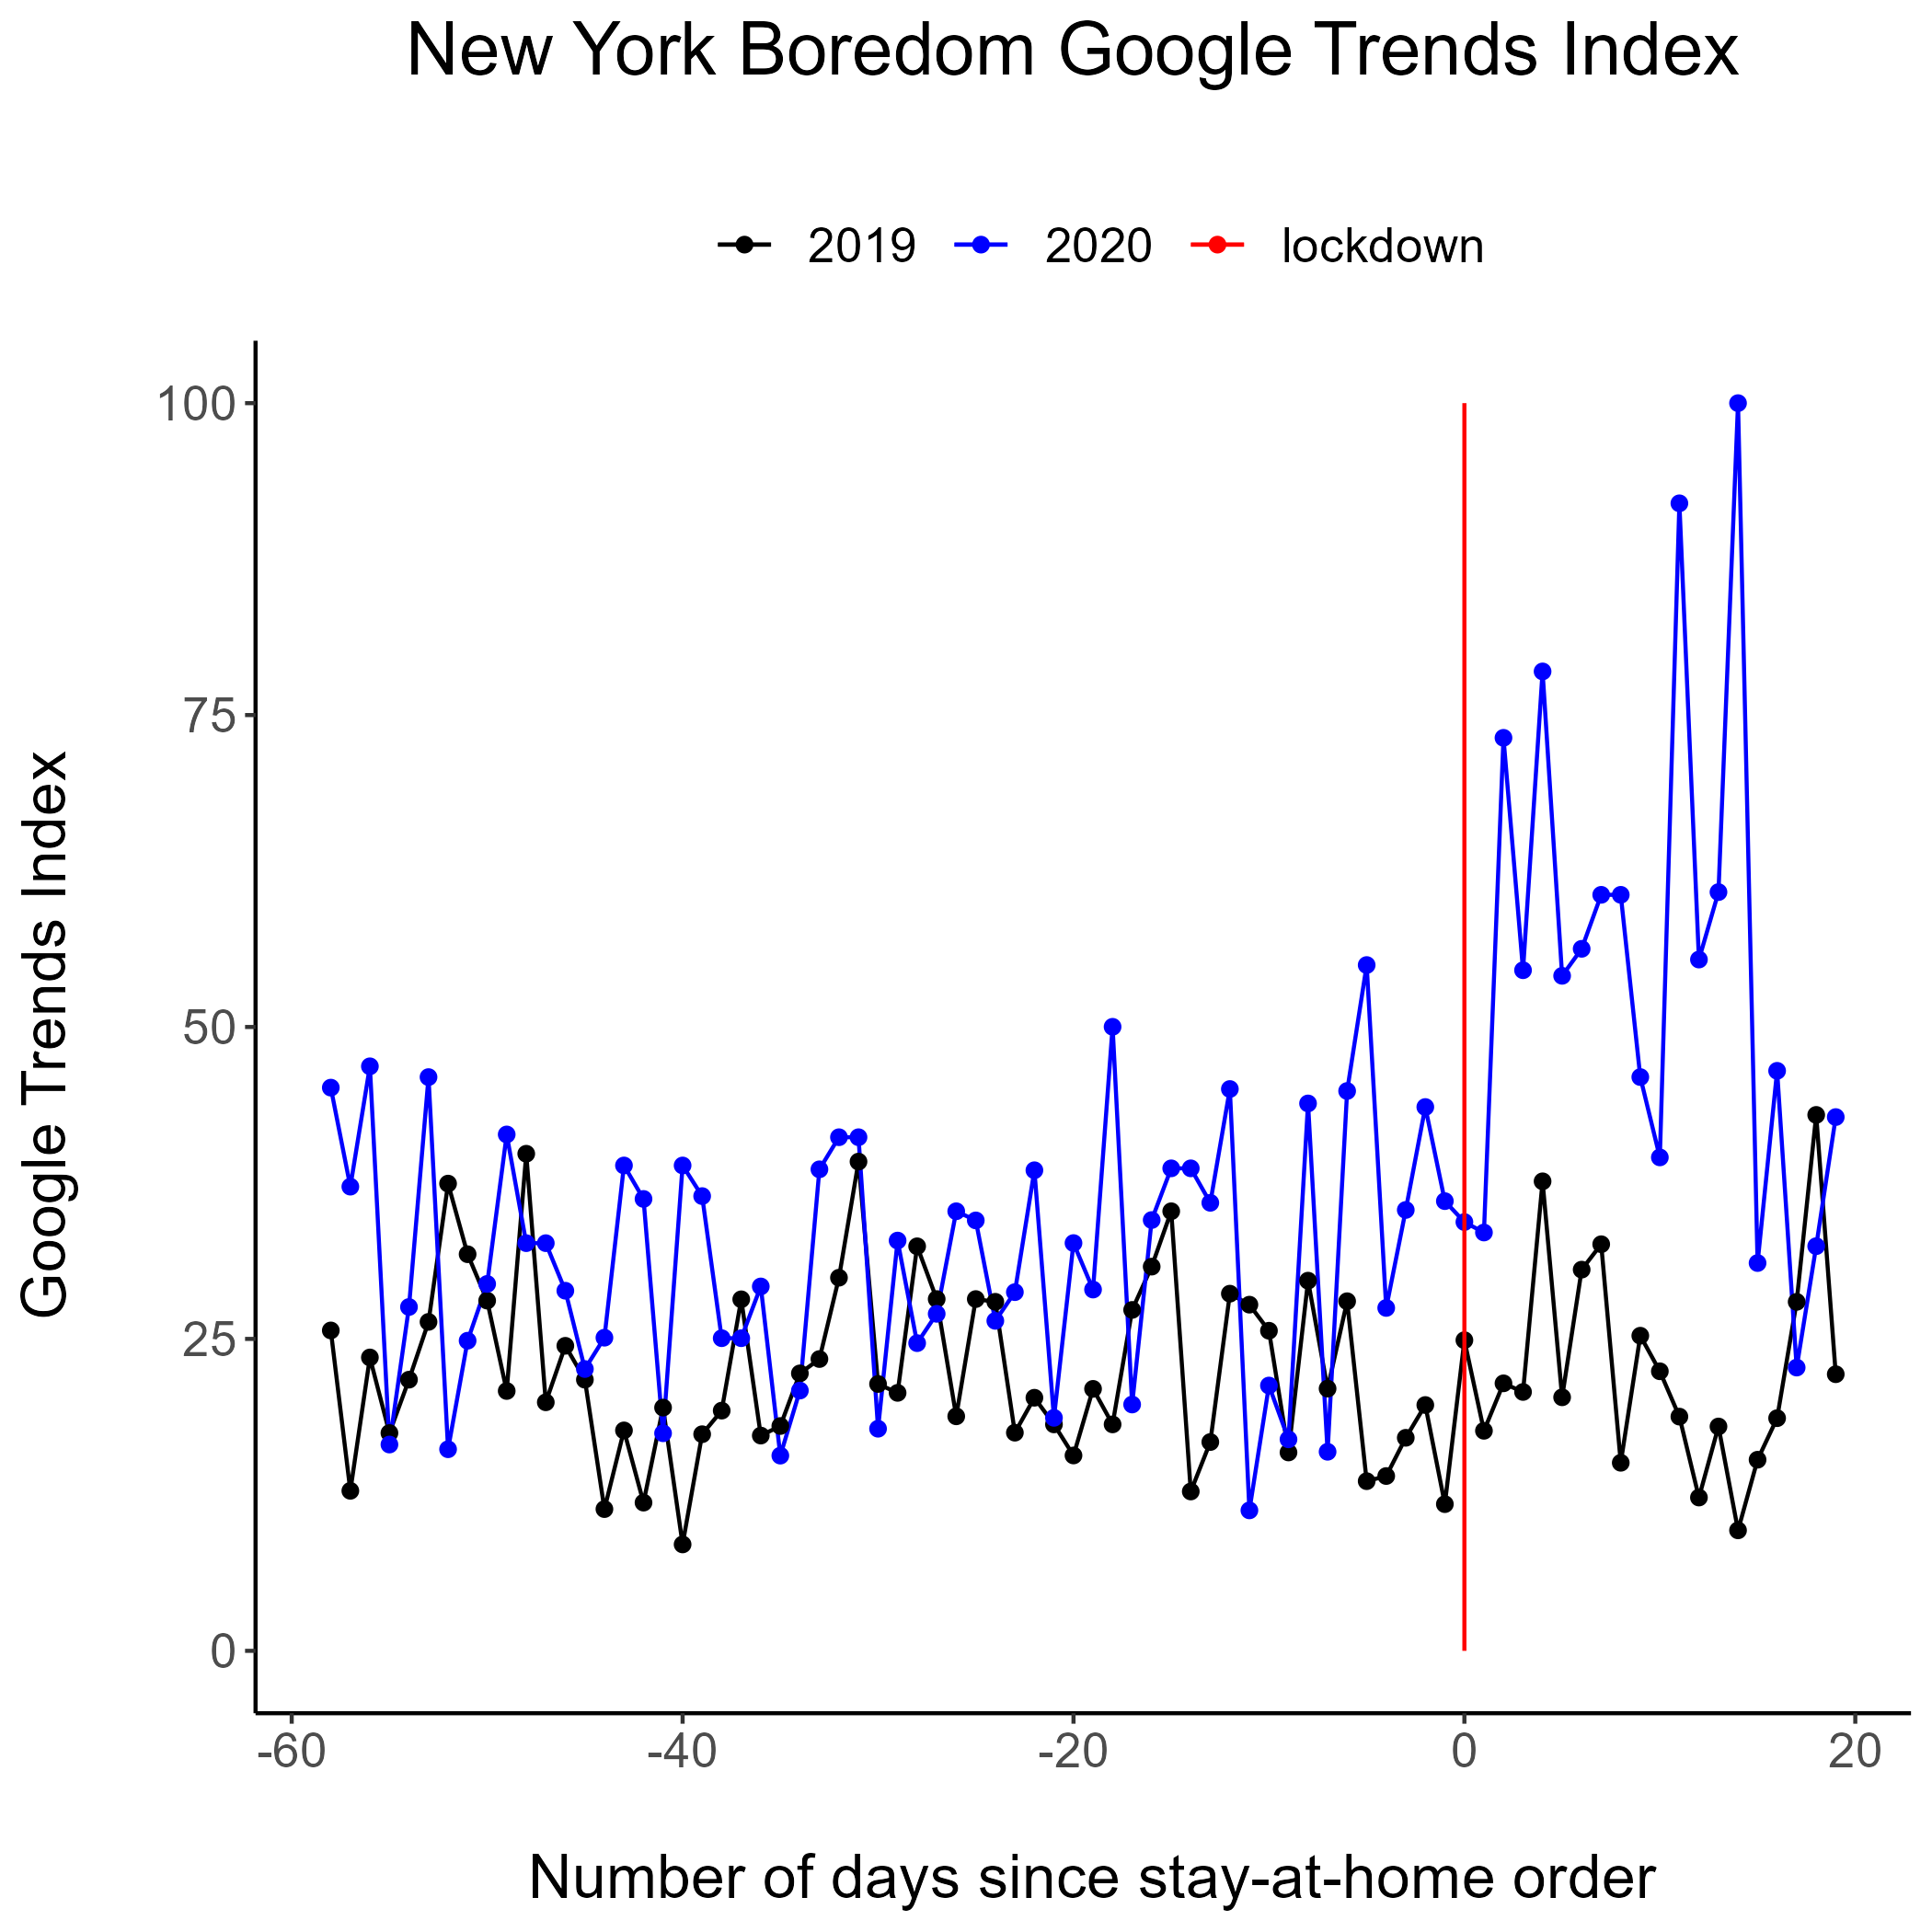
\includegraphics[clip, trim=0cm 0cm 0cm 0cm, width=0.6\textwidth]{Images/a6_q1_New Yorkboredom.png}
  \caption{Figure {\color{franklinblue} 2}: A Line Chart with Google Trends Data}
  \label{fig:linechart}
\end{figure}
\end{frame}

\begin{frame}[t]{Column, Bar, Pie and Bubble Charts}
\begin{description}
\item [Column Chart] Data that is arranged in columns or rows on a worksheet can be plotted in this type of  chart. This chart display categories along the horizontal (category) axis and values along the vertical (value) axis.
\item [Bar Chart] A chart that is a column chart where the categories are organized along the vertical axis, and the values along the horizontal axis.
\item [Pie Chart]  A chart that shows the size of items in one data series, proportional to the sum of the items. The data points in a such a chart are shown as a percentage of the entire area.
\item [Bubble Chart] A scatter chart where a third column is included that specifies the size of the bubbles/circles. 
\end{description}
\end{frame}

\begin{frame}[t]{Parallel-Coordinates Plot and Treemap}
\begin{description}
\item [Parallel-Coordinates Plot] This maps each row in a data table as a line, or profile. Each attribute of a row is represented by a point on the line. While these plots are similar in appearance to line charts, the way data is translated into a plot is substantially different.
\item [Treemap] This chart displays categories by color and proximity and can easily show lots of data which would be difficult with other chart types. The chart can be plotted when empty (blank) cells exist within the hierarchical structure.  This chart may be used to compare proportions within the hierarchy.
\end{description}
\end{frame}

\begin{frame}[t]{Scatter Plot Matrix, Heat Map and Sparkline}
\begin{description}
\item [Scatter Plot Matrix] This illustration is a grid (or matrix) of different charts, usually scatter charts, used to visualize bivariate relationships between combinations of variables. Each scatter plot in the matrix visualizes the relationship between a pair of variables, allowing many relationships to be explored in one chart.
\item [Heat Map] A table that depicts values for a main variable of interest across two axis variables as a grid of colored squares.
\item [Sparkline] A  very small line chart, typically drawn without axes or coordinates. It presents the general shape of the variation (typically over time) in some measurement, such as temperature, stock market price, sales, profits, \ldots in a simple and highly condensed way. 
\end{description}
\end{frame}

\begin{frame}[t]{A Scatter Matrix Example}
%https://tex.stackexchange.com/questions/114908/change-position-of-figure-in-beamer
\begin{figure}[htbp]
  \centering
  \captionsetup{justification=centering}
  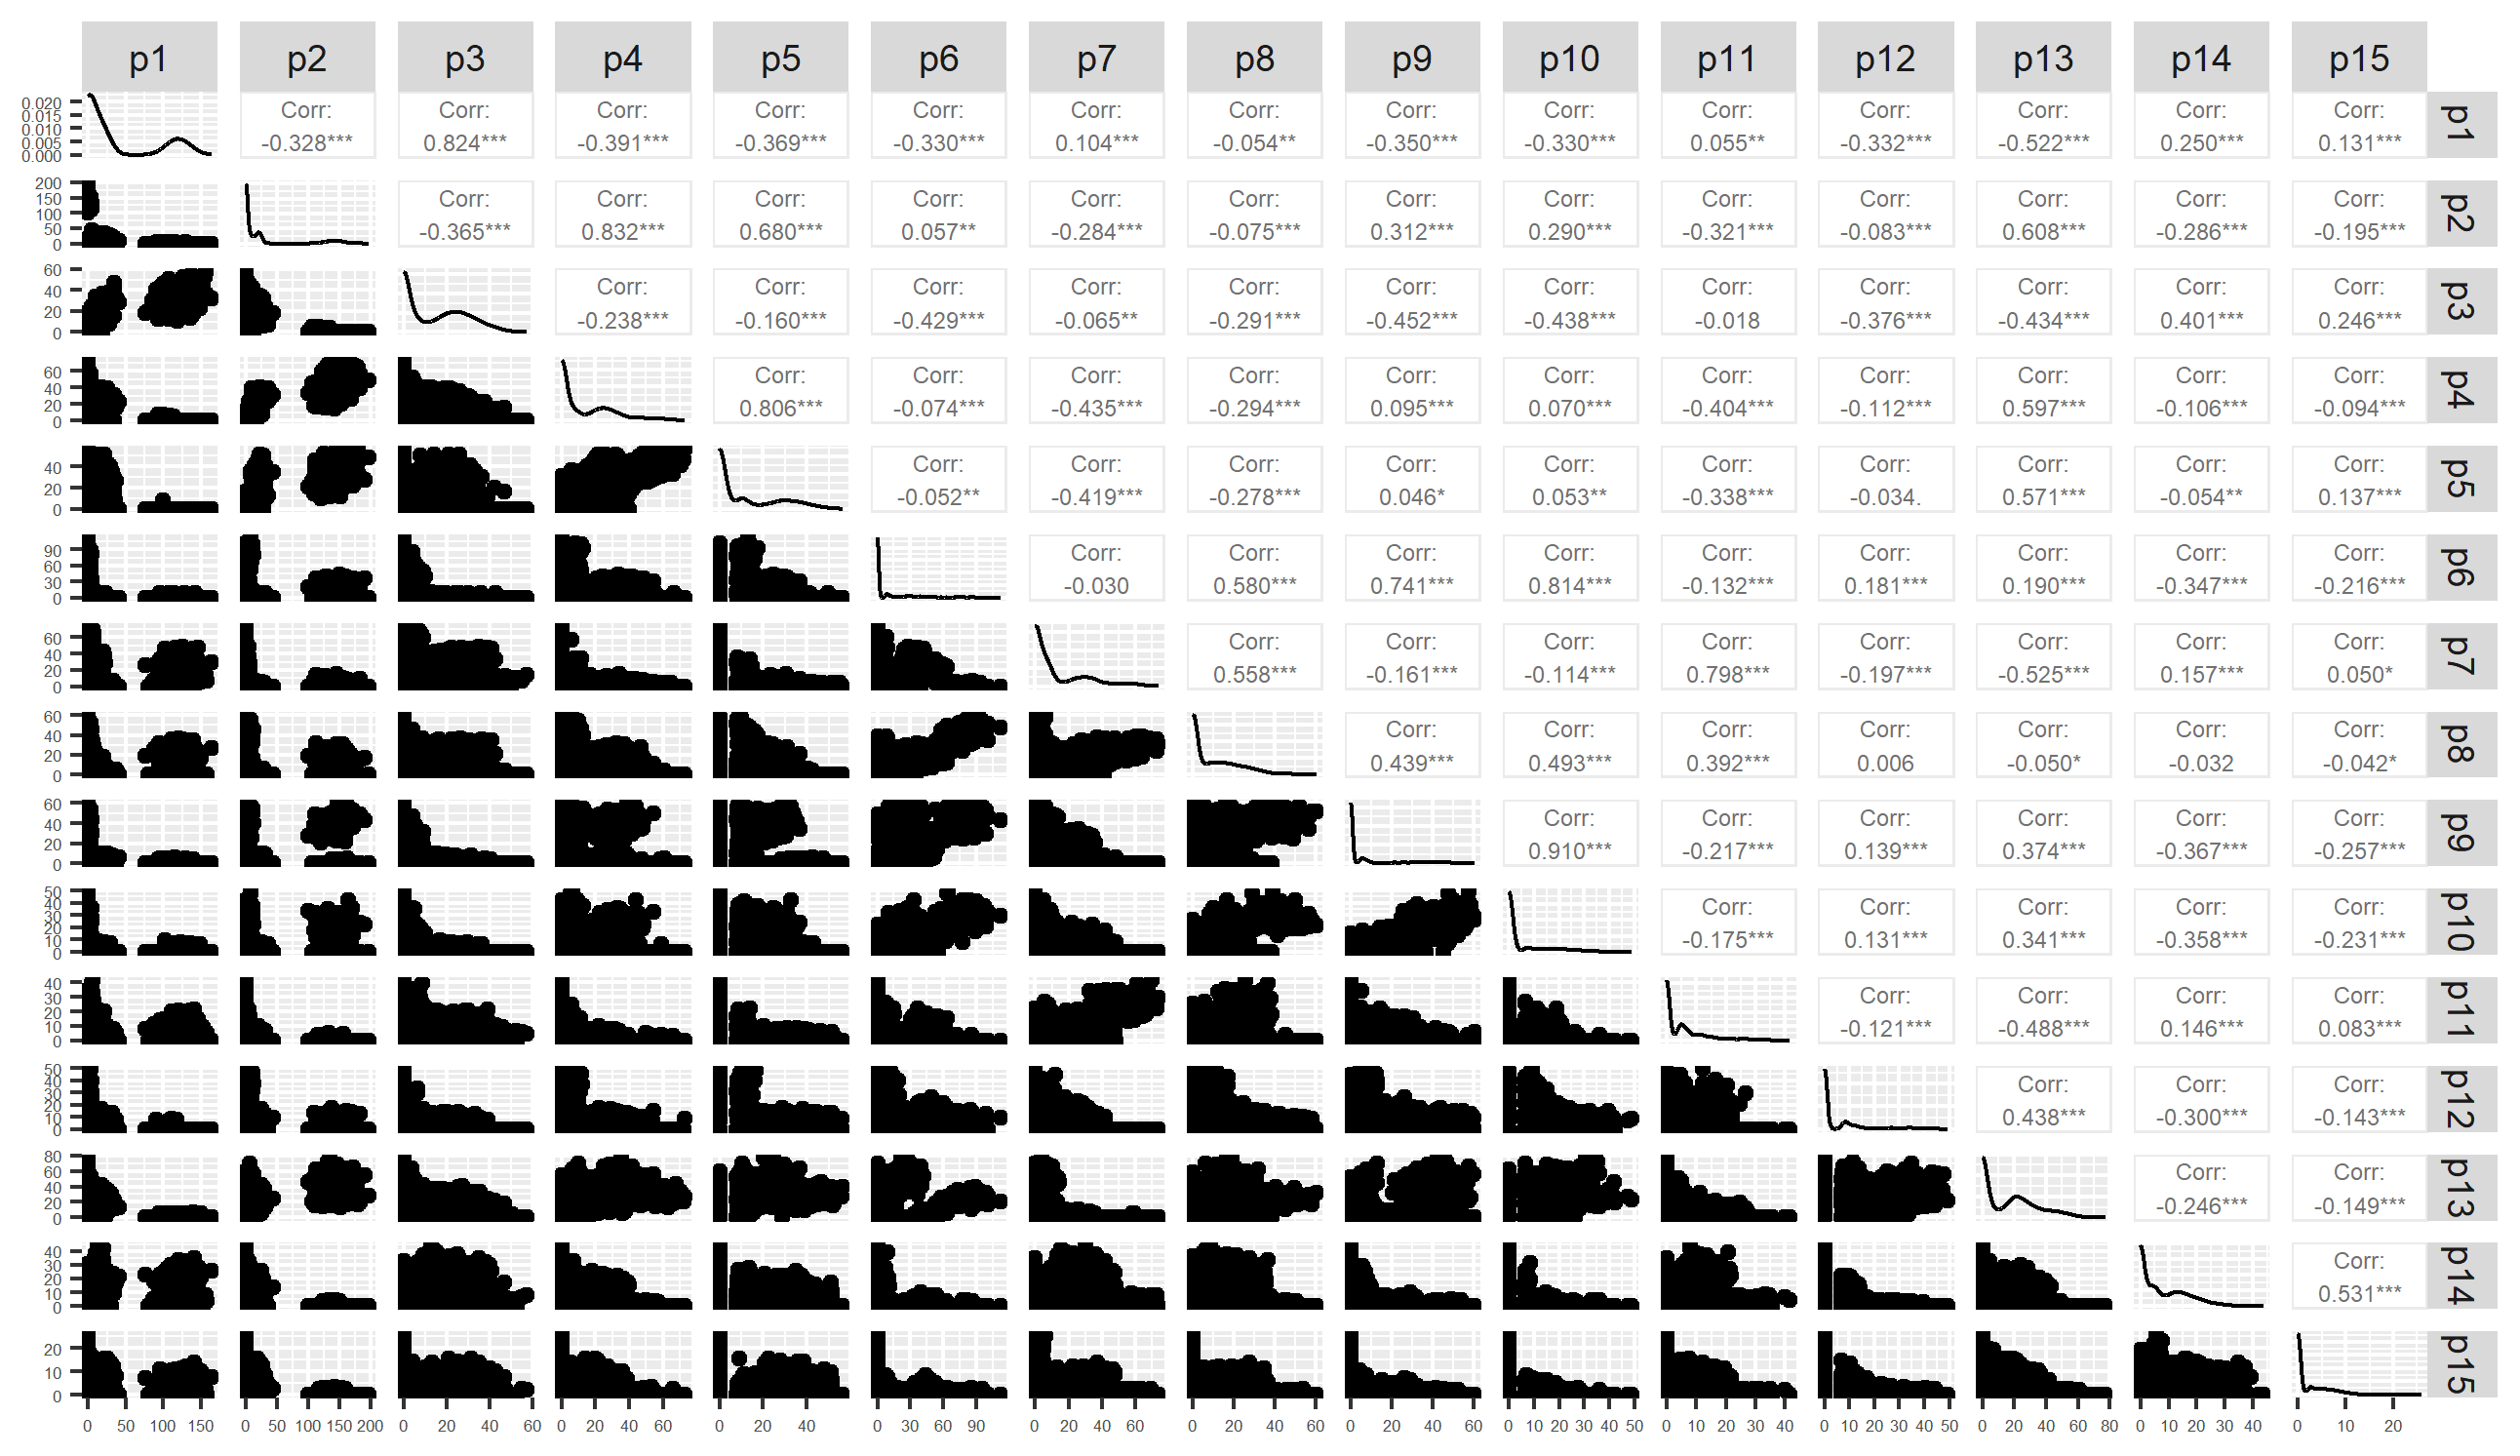
\includegraphics[clip, trim=0cm 0cm 0cm 0cm, width=1.0\textwidth]{Images/a3_q1f.png}
  \caption{Figure {\color{franklinblue} 3}: A Scatter Matrix \\ Bivariate Scatter Plots and Pearson Correlation Coefficients}
  \label{fig:scattermatrix}
\end{figure}
\end{frame}

\begin{frame}[t]{A Geographic Heat Map}
%https://tex.stackexchange.com/questions/114908/change-position-of-figure-in-beamer
\begin{figure}[htbp]
  \centering
  \captionsetup{justification=centering}
  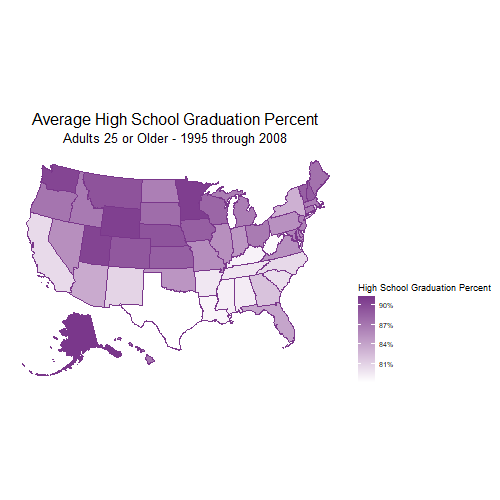
\includegraphics[clip, trim=0cm 3.5cm 0cm 3.5cm, width=1.0\textwidth]{Images/a7_q1d.png}
  \caption{Figure {\color{franklinblue} 4}: A Geographic Heat Map}
  \label{fig:geogheatmap}
\end{figure}
\end{frame}

\begin{frame}[t]{Rossmann}
The Excel file \texttt{daily\_store\_sales.xlsx} contains 2013 and 2014 daily store gross value sales in Euros, daily store customers, promotional information, store descriptions and other variables for the retailer \href{https://www.rossmann.de/de/}{Dirk Rossmann GmbH}, commonly referred to as Rossmann.\footnote{With the usual caveats about Wikipedia, \href{https://en.wikipedia.org/wiki/Rossmann_(company}{here} is the Wikipedia English language page about Rossmann.  The comma delimited file \texttt{daily\_store\_sales.csv} has the same data as the second tab of the aforementioned Excel file.}  \\
\vspace{1.5ex}
The retailer is one of the largest drug store chains in Europe with more than 45,000 employees and more than 4,000 stores in Germany, Poland, Hungary, Czechia, Turkey, Albania, Kosovo, and Spain.  \\
\vspace{0.5ex}
\small
\begin{itemize}
\item The tab \texttt{ReadMe\_First} of the Excel file has \empr{metadata}, a set of data that describes and gives information about other data, for the tab \texttt{daily\_store\_sales}.
\end{itemize}
\end{frame}

\begin{frame}[t]{Data Differences}
\small
\begin{itemize}
\item Excel's \texttt{Pivot Table} functionality may be used to summarize the data, where the resulting data may be used to create charts. 
\end{itemize}
\vspace{-1.5ex}
\normalsize
Suppose the data is maintained in marketing staging and production databases.\footnote{A staging database is a parallel data warehouse database that stores data temporarily while it is loaded into the appliance that maintains the production database. The primary benefit of a staging database is to reduce table fragmentation, and hence results in faster queries.}  These databases are different than the SAP financial database used by the Rossmann finance department.  \\
\vspace{1.5ex}
At a meeting yesterday afternoon the CMO was discussing some sales charts and tables with the CFO.  Upon a careful review of these charts and tables, the CFO told the CMO that the data he presented may not be correct. As you may expect, the CMO was not particularly happy with this revelation. \\
\end{frame}

\begin{frame}[t]{A Call to Action!}
The CMO has requested your and your fellow marketing department colleagues to investigate the CFO's claim.  \\
\vspace{0.0ex}
\small
\begin{itemize}
\item Specifically, he has asked you to populate the charts on the next 5 slides using \texttt{daily\_store\_sales}.  The charts and their input data will be compared and contrasted to like information begin obtained by the Rossmann Information Technology department.  If you notice any anomalies in the data, or insightful marketing analytic insigts, you are to mention it.  
\item While you and your colleagues may use Excel, Python, R, \ldots to create the charts, the data used to create the charts must be made available in either Excel or Google Sheets.
\item Time is of the essence since in a few weeks the marketing database will be undergoing its annual lockdown development period.\footnote{The marketing production and staging databases will not have any table, view, production queries \ldots, revisions created, tested, and deployed. The lockdown ensures resources are readily available to meet end of fiscal year reporting needs.} 
\end{itemize} 
\end{frame}

\begin{frame}[t]{Total Sales and Total Customer Visits Scatter Plot}
\begin{figure}[htbp]
    \centering
    \captionsetup{justification=centering}
    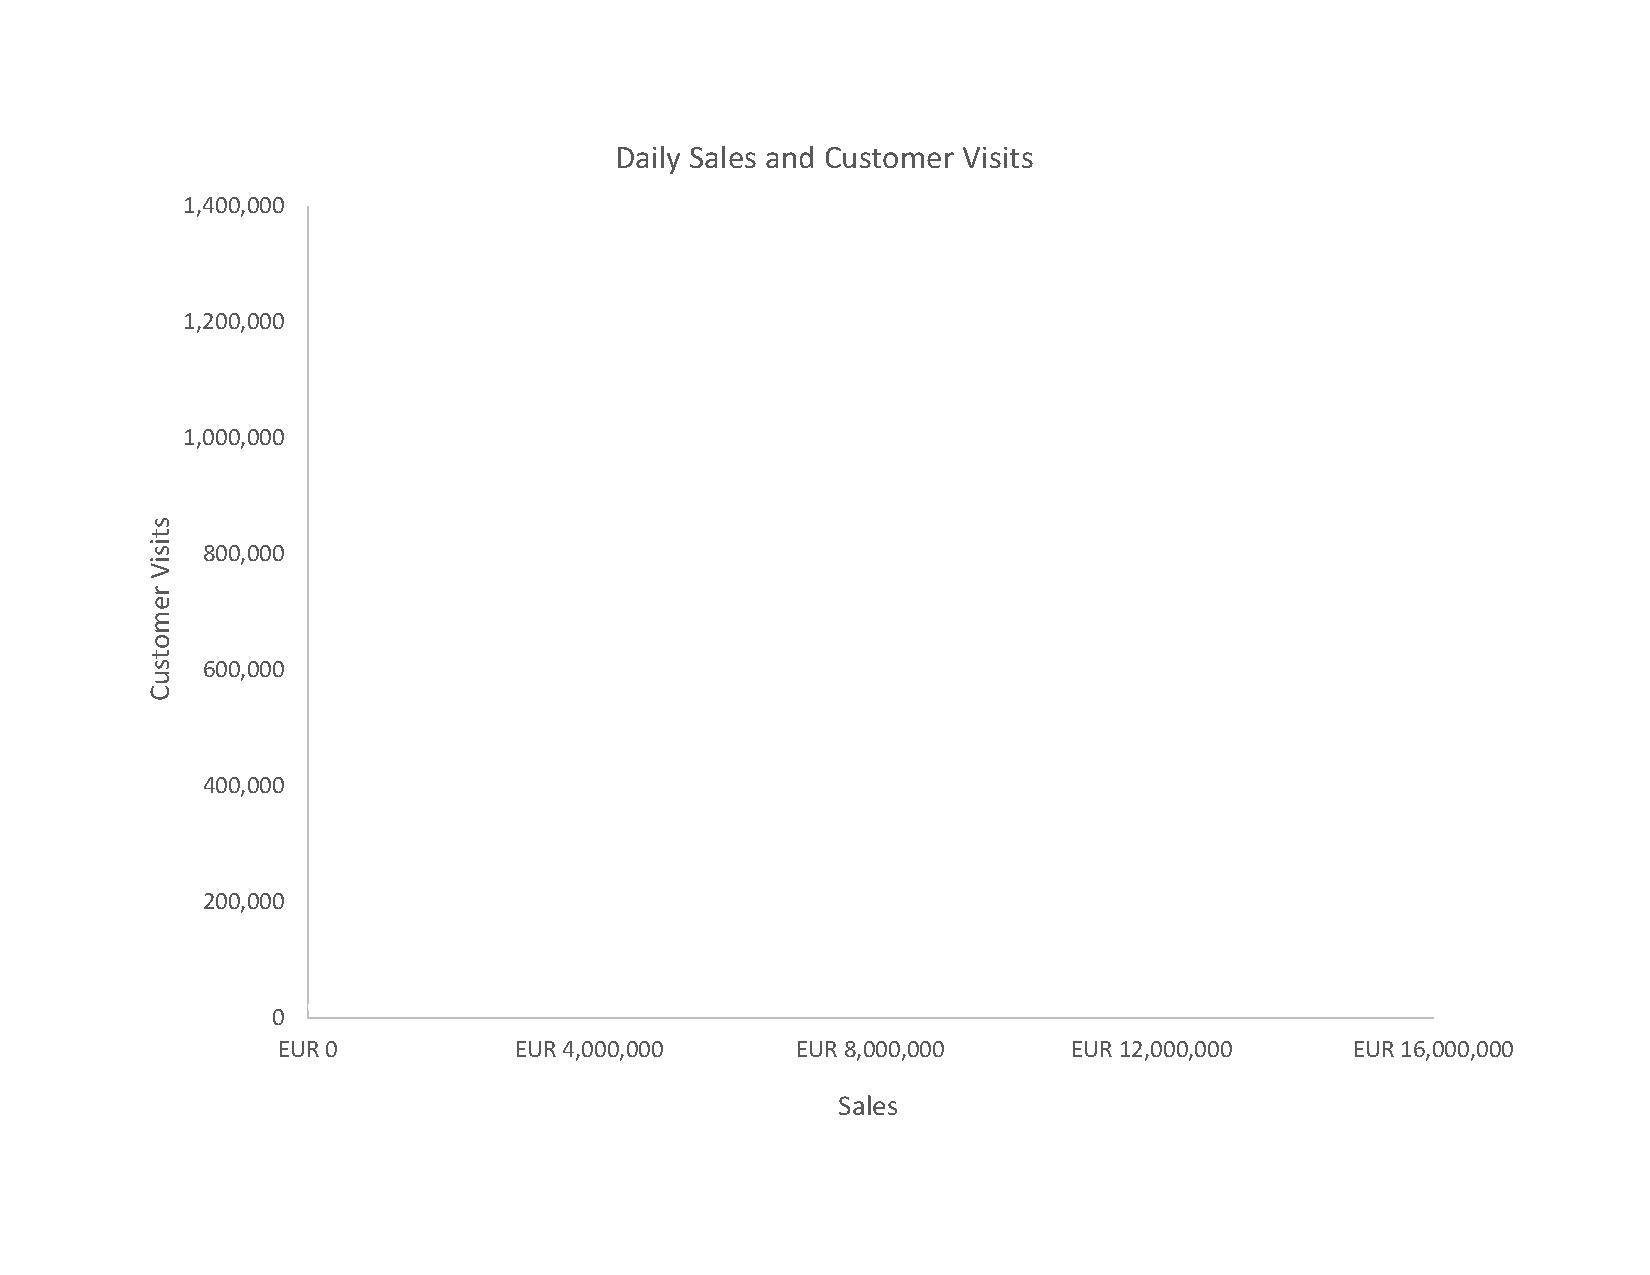
\includegraphics[clip, trim=0cm 2.3cm 0cm 2.3cm, width=1.0\textwidth]{Scatter_Plot_Unit_3_Template.pdf}  
    \caption{Figure {\color{franklinblue} 5}: Daily Sales and Customer Visits Scatter Plot Template}
    \label{fig:scatter0}
\end{figure}
\end{frame}

\begin{frame}[t]{Sales and Customer Visits Time Series Chart}
\begin{figure}[htbp]
    \centering
    \captionsetup{justification=centering}
    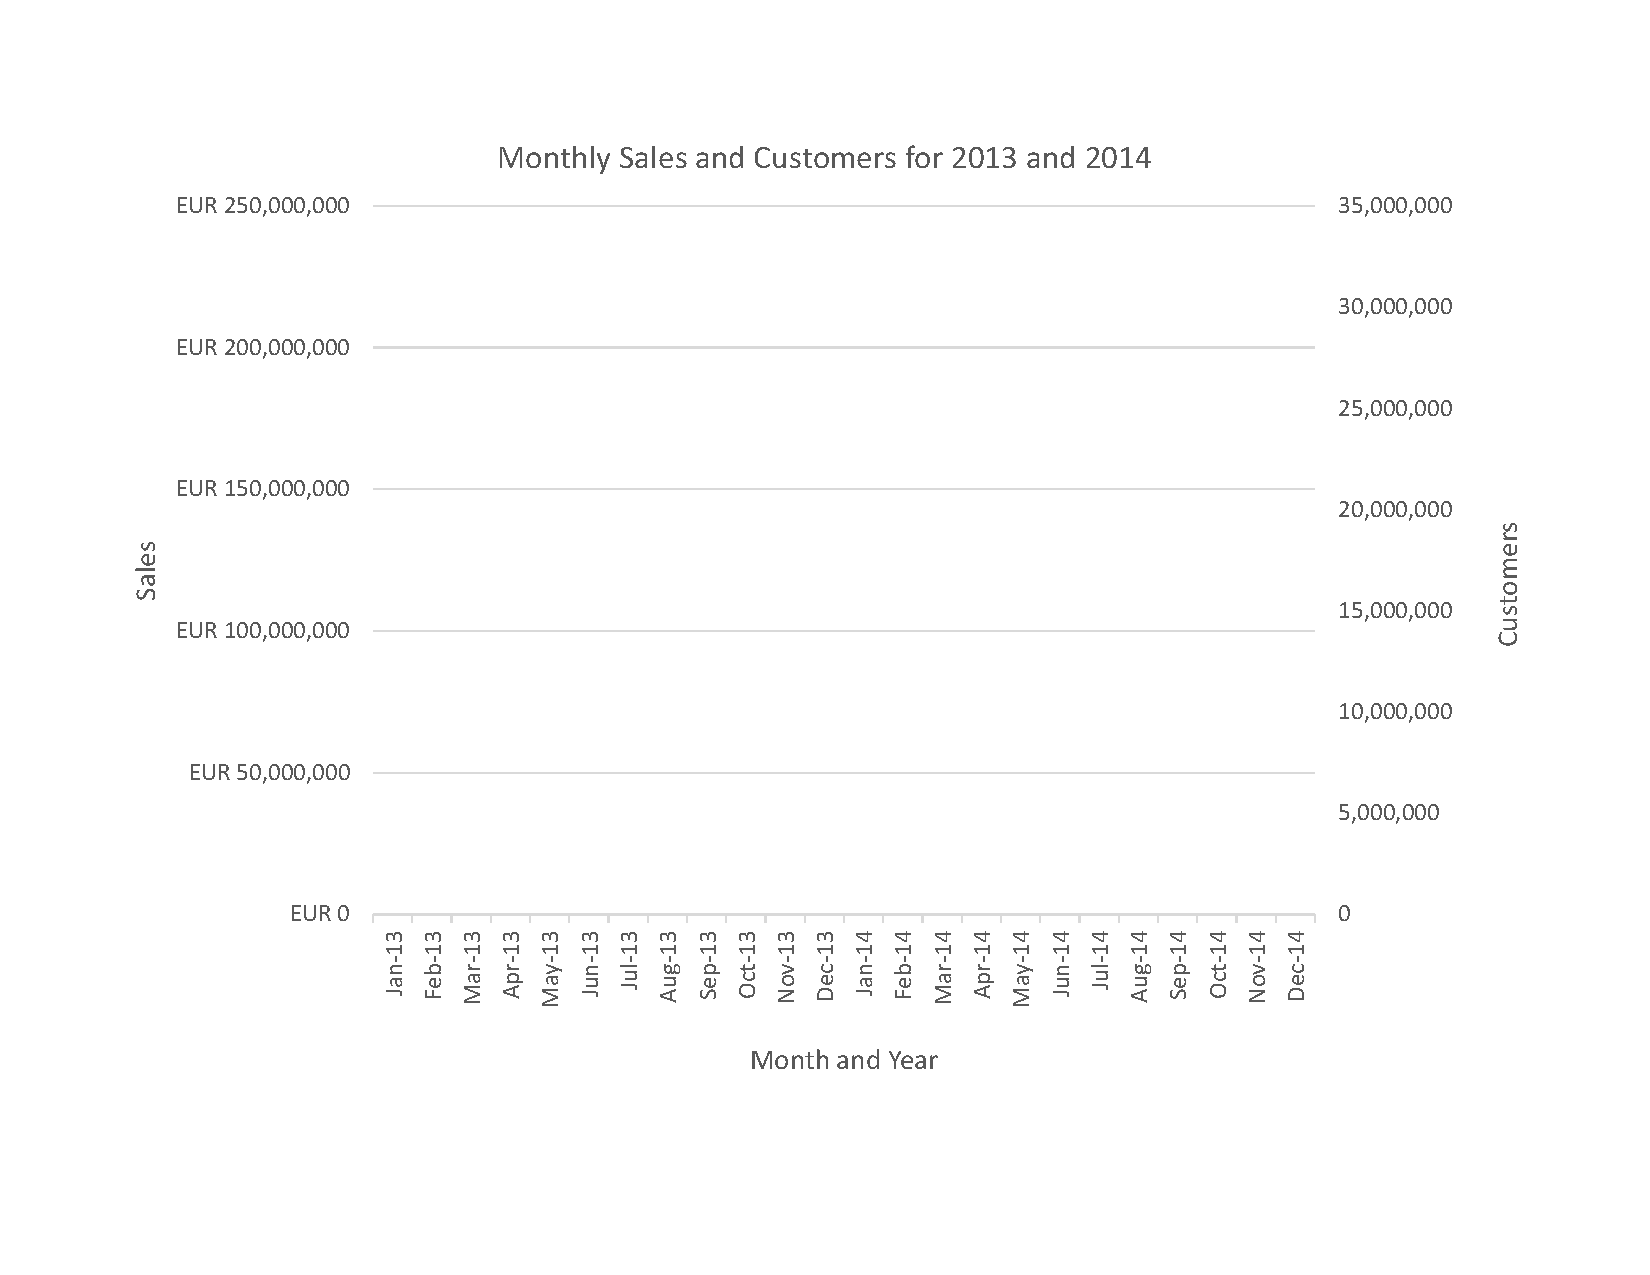
\includegraphics[clip, trim=0cm 2.3cm 0cm 2.3cm, width=1.0\textwidth]{Line_Chart_Unit_3_Template.pdf}
    \caption{Figure {\color{franklinblue} 6}: Monthly Sales and Customer Visits for 2013 and 2014 Time Series Chart Template}
    \label{fig:linechart0}
\end{figure}
\end{frame}

\begin{frame}[t]{Store Type and Assortment Bar Chart}
\begin{figure}[htbp]
    \centering
    \captionsetup{justification=centering}
    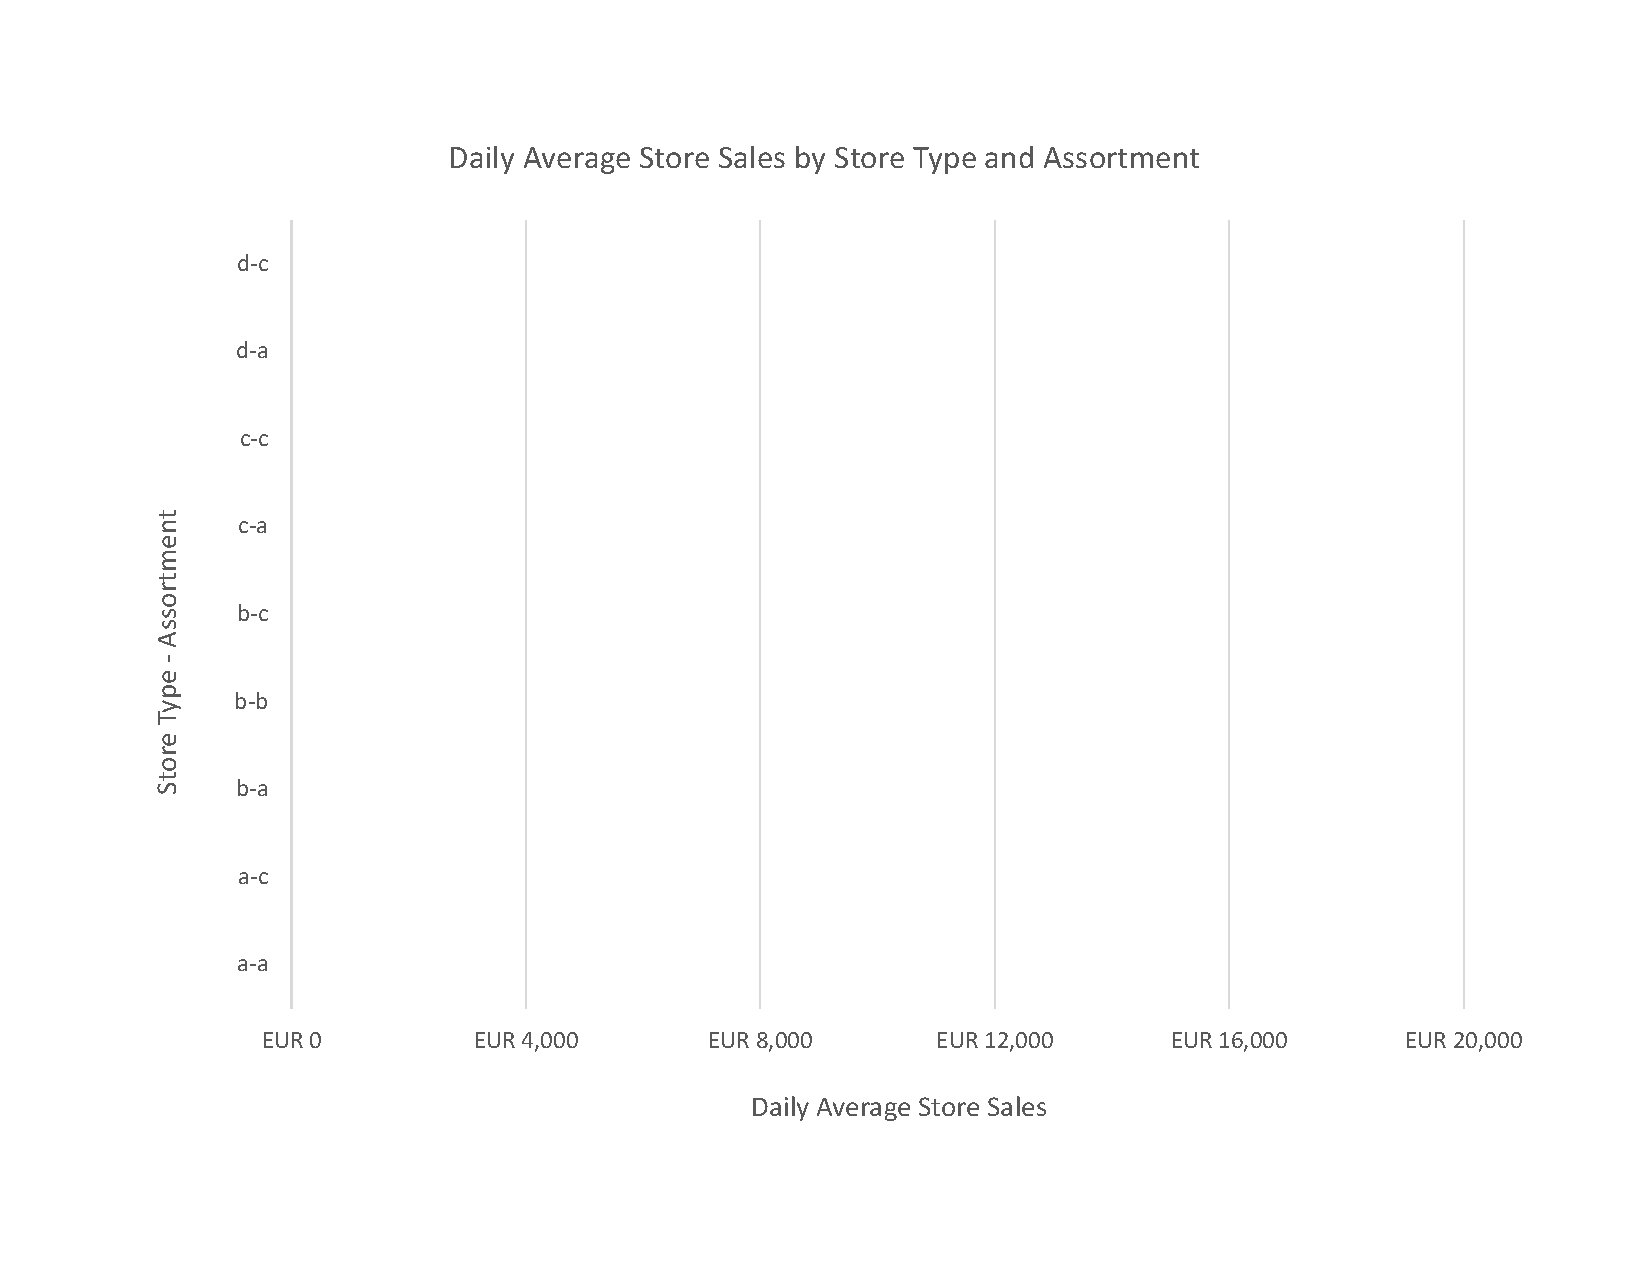
\includegraphics[clip, trim=0cm 2.3cm 0cm 2.3cm, width=1.0\textwidth]{Bar_Chart_Unit_3_Template.pdf}  
    \caption{Figure {\color{franklinblue} 7}: Daily Average Store Sales by Store Type and Assortment Bar Chart Template}
    \label{fig:barchart0}
\end{figure}
\end{frame}

\begin{frame}[t]{Store Type and Assortment Bubble Chart}
\begin{figure}[htbp]
    \centering
    \captionsetup{justification=centering}
    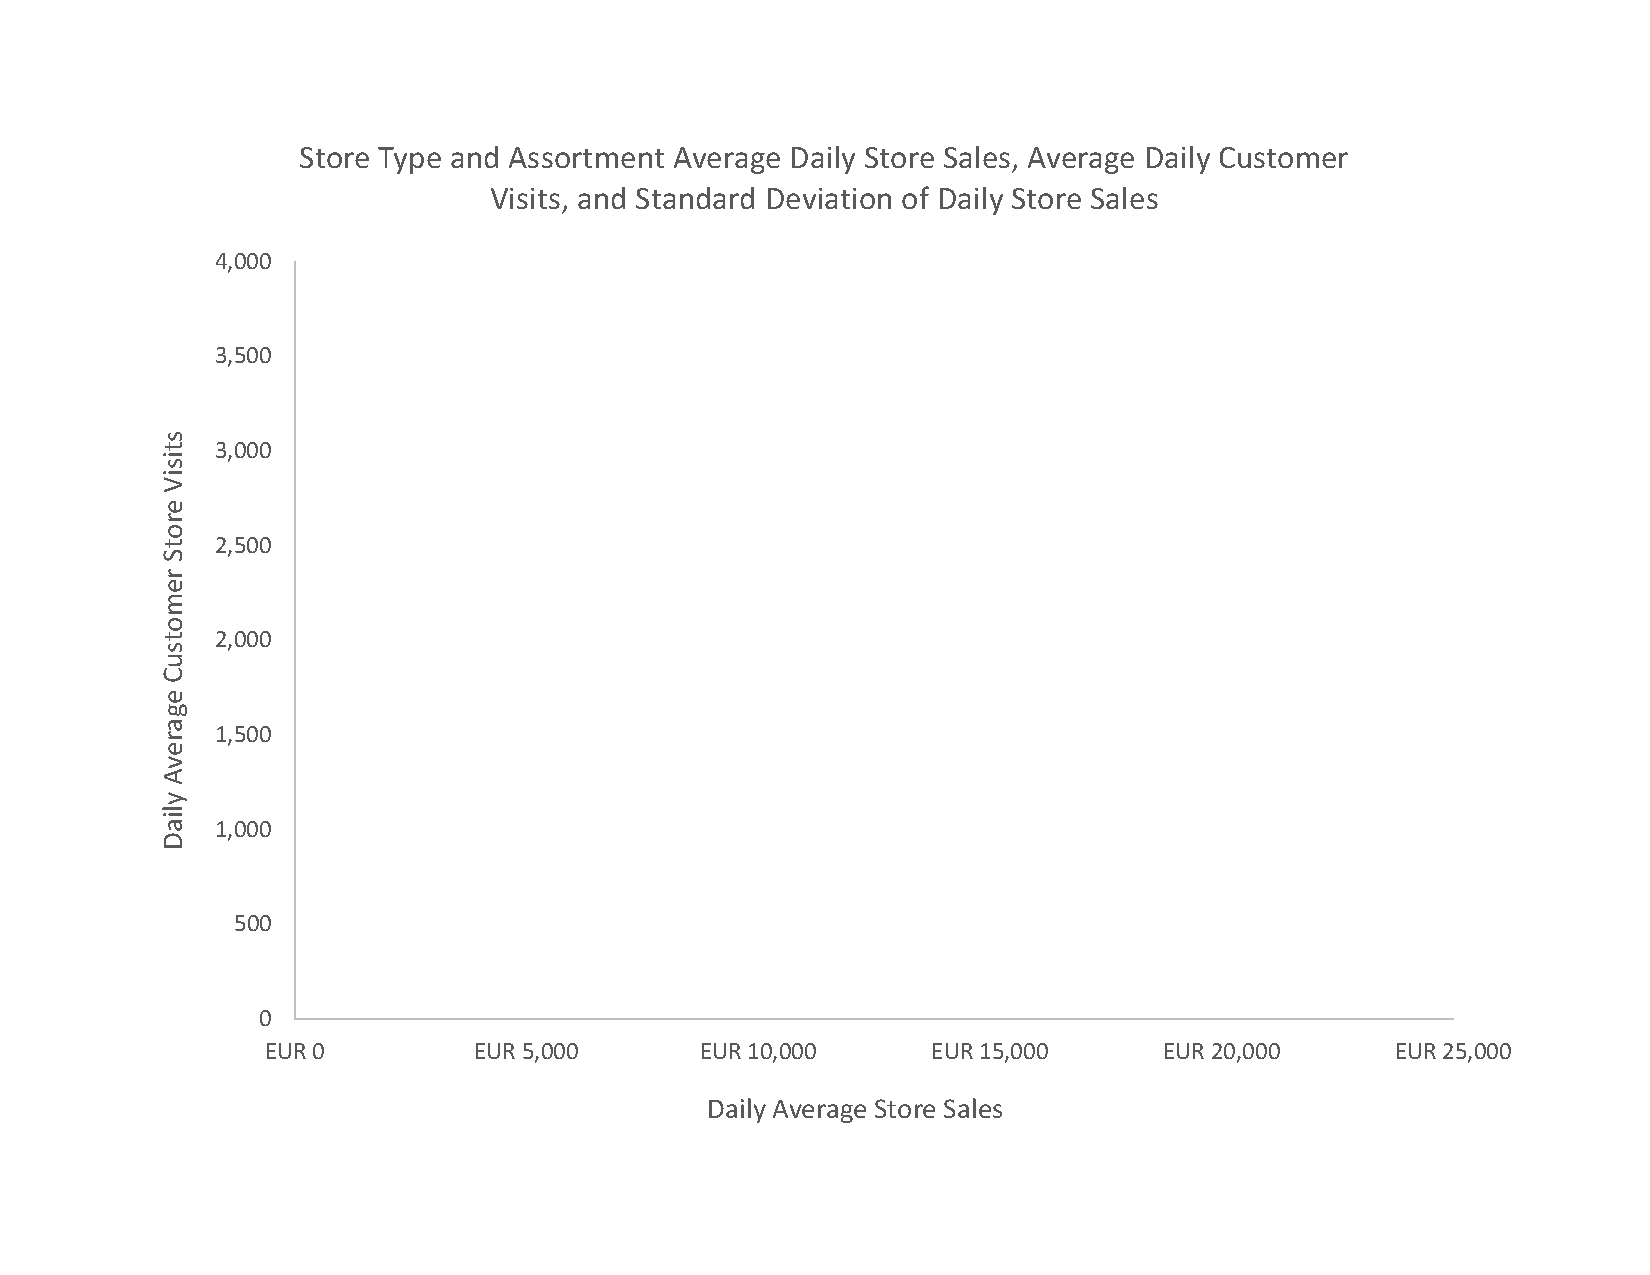
\includegraphics[clip, trim=0cm 2.3cm 0cm 2.3cm, width=0.8\textwidth]{Bubble_Chart_Unit_3_Template.pdf}  
    \caption{Figure {\color{franklinblue} 8}: Store Type and Assortment Average Daily Store Sales, Average Daily Customer Visits, and Standard Deviation of Daily Store Sales Bubble Chart Template}
    \label{fig:bubblechart0}
\end{figure}
\vspace{-2.0ex}
\small
The standard deviation of daily store sales are used for bubble size. 
\end{frame}

\begin{frame}[t]{Store Type Monthly Sales \% Change Heat Map}
\begin{figure}[htbp]
    \centering
    \captionsetup{justification=centering}
    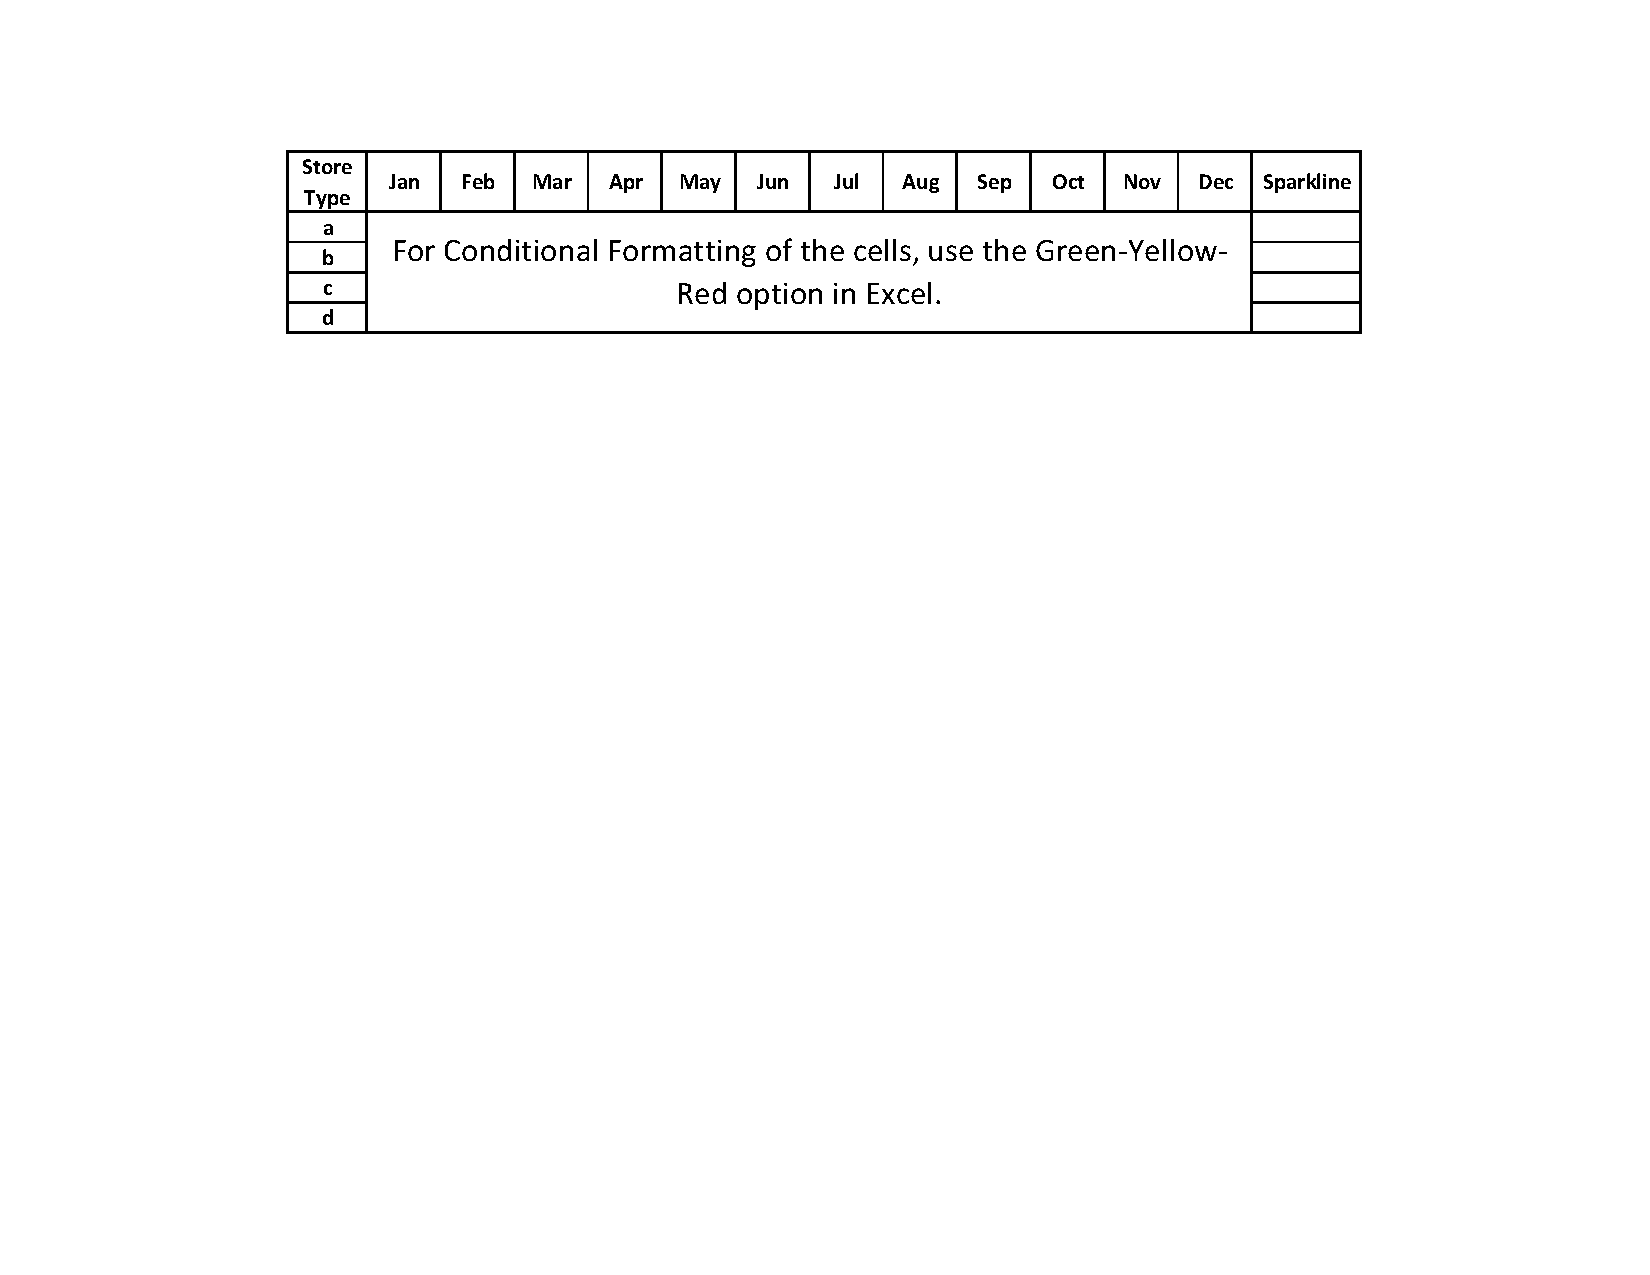
\includegraphics[clip, trim=4.9cm 15.5cm 0cm 2.5cm, width=1.25\textwidth]{Heat_Map_Unit_3_Template.pdf}  
    \caption{Table {\color{franklinblue} 1}: Store Type Monthly Sales Percentage Change Heat Map Template}
    \label{fig:heatmap0}
\end{figure}
\end{frame}

\section{References}

\begin{frame}[t,allowframebreaks]
%https://latex-beamer.com/faq/long-bibliographies-beamer/
%https://github.com/jgm/pandoc/issues/2442
\widowpenalties 1 10000
\small
\bibliography{../../Bibliography/list2}
\bibliographystyle{apalike}
\end{frame}

\end{document}